\chapter{Background}
\label{chapter2}
%\setlength{\epigraphrule}{0pt}
\epigraph{\textit{We can draw lessons from the past, but we cannot live in it.}}{ -- Lyndon B. Johnson}

% **************************** Define Graphics Path **************************
\ifpdf
    \graphicspath{{Chapter2/Figs/Raster/}{Chapter2/Figs/PDF/}{Chapter2/Figs/}}
\else
    \graphicspath{{Chapter2/Figs/Vector/}{Chapter2/Figs/}}
\fi


\section{TRECVID Multimedia Event Detection}

As introduced in Chapter \ref{chapter1}, complex event recognition is an important computer vision research with many potential applications. In 2010 TRECVID community has proposed a new task, named ``Multimedia Event Detection'' to advance the research and development in this area. The ultimate purpose of this task is to collect technologies for building a computer system that can quickly search for a particular event over a large video collection. \index{trecvid} \index{multimedia event detection}
 
The task is defined as follows: ``Given an event kit, find all clips that contain the event in a video collection'' \cite{over2011trecvid}. The event kit provides the event definitions along with some example videos of each event. At first, MED task defines an event:\textit{ is a complex activity occurring at a specific place and time; involves people interacting with other people and/or objects; consists of a number of human actions, processes, and activities that are loosely or tightly organized and that have significant temporal and semantic relationships to the overarching activity; and is directly observable}. 

For a specific event of interest, a textual description is also provided to help developers generate the event search query. This textual description consists of following information: event name, event definition, event explication and evidential description. The event name is a mnemonic title of that event. The event definition provides a short definition of that event. Event explication is a long description which explains ambiguous terminologies in the event definition. Finally, the evidential description summarizes an event with its characteristics such as scene, object/people, activities and audio information. Table \ref{c2_eventkit} shows textual description of an event in MED task.

% Please add the following required packages to your document preamble:
% \usepackage{booktabs}

\begin{table}[h]
	\centering	
	\caption{Textual description for event ``Attempting a board trick''}
	\renewcommand{\arraystretch}{1.5}	
	\begin{tabular}{|l|l|}
		\hline
		Event name             & Attempting a board trick                                                                                                                                                                                                                                                                                                                                                                                                                                                                                                                                                                                                                                                                  \\ \hline
		Definition             & \begin{tabular}[c]{@{}l@{}}One or more people attempt to do a trick on a skateboard, snowboard, \\ surfboard, or other boardsport board.\end{tabular}                                                                                                                                                                                                                                                                                                                                                                                                                                                                                                                                     \\ \hline
		Explication            & \begin{tabular}[c]{@{}l@{}}Board sports are sports where a person stands, sits, or lays on a board \\ and moves and controls the board. Tricks consist of intentional motions\\ made with the board that are not simply slowing down/stopping the board \\ or steering the board as it moves. Steering around obstacles or steering a \\ board off of a jump and landing on the ground are not considered tricks in \\ and of themselves.\\ Common tricks involve actions like sliding the board along the top of an\\ object (e.g. a swimming pool rim or railing), jumping from the ground or\\ the surface of water into the air, and spinning or flipping in the air.\end{tabular} \\ \hline
		\begin{tabular}[c]{@{}l@{}}Evidential \\ description\end{tabular} & \begin{tabular}[c]{@{}l@{}}\textbf{scene}: outside, often in a skate park.\\ \textbf{objects/people}: skateboard, snowboard, surfboard, ramps, rails, safety\\ gear, crowds.\\ \textbf{activities}: standing, sitting or laying on the board; jumping with the board; \\ flipping the board and landing on it; spinning the board; sliding the board \\ across various objects.\\ \textbf{audio}: sounds of board hitting surface during trick; crowd cheering.\end{tabular}                                       \\ \hline
	\end{tabular}
	\label{c2_eventkit}
\end{table}



\section{Datasets}
There are only three events that are being tested in the pilot year (MED 2010\footnote{http://www.nist.gov/itl/iad/mig/med10.cfm}). These events are the following:
(1) ``Assembling a shelter'': one or more people construct a temporary or semi-permanent shelter for humans that could provide protection from the elements.
(2) ``Batting a run in'': within a single play during a baseballtype game, a batter hits a ball and one or more runners (possibly including the batter) scores a run.
And (3) ``Making a cake'': One or more people make a cake.

Since 2011, the number of test events has been increasing. New tested events as well as tested videos are added every year. For example, there are 5 training events (E001-E005) and 10 testing events (E006-E015) in MED 2011\footnote{http://www.nist.gov/itl/iad/mig/med11.cfm}. The number for MED 2012 is 20 testing events (E006-E015, E021-E030)\footnote{http://www.nist.gov/itl/iad/mig/med12.cfm}. These events are also kept in MED 2013 but more testing videos are added. In MED 2014, a different test set with 10 new events are introduced (E021-E040). List of all event names up to TRECVID MED 2014 can be found in Table \ref{c2_eventlist}. Since MED 2012, the evaluation set which contains around 98,000 test videos has been frozen. This collection is blind to all participants, which means they are not allowed to analyze these videos when tuning their systems. 
In MED 2014 the evaluation set was doubled by adding around 100,000 test videos. An overview of all MED video collections is shown in Table \ref{c2_dataset}. To the best of our knowledge, this is largest video dataset for event detection purpose. Since 2012, the evaluation dataset is frozen. Therefore, most researchers conducts experiments on MED2010, MED2011 and MED2012 dataset. The detail information of these dataset can be seen in \ref{c2_exp_dataset}.

% Please add the following required packages to your document preamble:
% \usepackage{booktabs}
% \usepackage{multirow}
% Please add the following required packages to your document preamble:
% \usepackage{booktabs}
% \usepackage{multirow}
\begin{table}[h]
	\centering
	\caption{Number of videos duration in MED dataset up to 2014.}
	\begin{tabular}{@{}|c|l|c|c|@{}}
		\toprule
		\multicolumn{2}{|c|}{Set}                                                                         & Number of video clips & Video duration (hours) \\ \midrule
		\multirow{3}{*}{\begin{tabular}[c]{@{}c@{}}Development\\ Data\end{tabular}}    & RESEARCH         & 10,000                & 314                    \\ \cmidrule(l){2-4} 
		& 10 Event Kits    & 1,400                 & 74                     \\ \cmidrule(l){2-4} 
		& Transcription    & 1,500                 & 45                     \\ \midrule
		\multirow{2}{*}{\begin{tabular}[c]{@{}c@{}}Event\\ Training Data\end{tabular}} & Event Background & 5,000                 & 146                    \\ \cmidrule(l){2-4} 
		& 40 Event Kits    & 6,000                 & 270                    \\ \midrule
		\multirow{2}{*}{Test Data}                                                     & MEDTest          & 27,000                & 849                    \\ \cmidrule(l){2-4} 
		& KindredTest      & 14,500                & 687                    \\ \midrule
		\multirow{2}{*}{Evaluation Data}                                               & MED14Eval-Full   & 198,000               & 7,580                  \\ \cmidrule(l){2-4} 
		& MED14Eval-Sub    & 33,000                & 1,244                  \\ \midrule
		\multicolumn{2}{|c|}{Total}                                                                       & 244,000               & 9,911                  \\ \bottomrule
	\end{tabular}
	\label{c2_dataset}
\end{table}

% Please add the following required packages to your document preamble:
% \usepackage{booktabs}
\begin{table}[h]
		\centering
		\caption{Detail information of MED2010, MED2011 and MED2012 dataset.}
	\begin{tabular}{@{}lccccc@{}}
		\toprule
		\multicolumn{1}{c}{Dataset} & No. Event & No. Train Videos & No. Test Videos & Total Videos & Total Hours \\ \midrule
		MED2010                     & 3         & 1,744            & 1,724           & 3,468        & 110 hours   \\
		MED2011                     & 10        & 1,331            & 31,822          & 33,153       & 1,100 hours \\
		MED2012                     & 25        & 3,878            & 1,938           & 5,816        & 250 hours   \\ \bottomrule
	\end{tabular}
	\label{c2_exp_dataset}
\end{table}

\begin{table}
	\centering
	\caption{List of event names in MED task from 2010-2014.}	
	\renewcommand{\arraystretch}{1.5}		
	\begin{tabular}{@{}|c|l|l|l|@{}}
		\toprule
		\textbf{ID}                & \multicolumn{1}{c|}{\textbf{Event name}} & \textbf{ID} & \textbf{Event name}               \\ \midrule
		E001                       & Attempting a board trick                 & E021        & Attempting a bike trick           \\ \midrule
		E002                       & Feeding an animal                        & E022        & Cleaning an appliance             \\ \midrule
		E003                       & Landing a fish                           & E023        & Dog show                          \\ \midrule
		E004                       & Wedding ceremony                         & E024        & Giving directions to a location   \\ \midrule
		E005                       & Working on a woodworking project         & E025        & Marriage proposal                 \\ \midrule
		E006                       & Birthday party                           & E026        & Renovating a home                 \\ \midrule
		E007                       & Changing a vehicle tire                  & E027        & Rock climbing                     \\ \midrule
		E008                       & Flash mob gathering                      & E028        & Town hall meeting                 \\ \midrule
		E009                       & Getting a vehicle unstuck                & E029        & Winning a race without a vehicle  \\ \midrule
		E010                       & Grooming an animal                       & E030        & Working on a metal crafts project \\ \midrule
		\multicolumn{1}{|l|}{E011} & Making a sandwich                        & E031        & Beekeeping                        \\ \midrule
		\multicolumn{1}{|l|}{E012} & Parade                                   & E032        & Wedding shower                    \\ \midrule
		\multicolumn{1}{|l|}{E013} & Parkour                                  & E033        & Non-motorized vehicle repair      \\ \midrule
		\multicolumn{1}{|l|}{E014} & Repairing an appliance                   & E034        & Fixing musical instrument         \\ \midrule
		\multicolumn{1}{|l|}{E015} & Working on a sewing project              & E035        & Horse riding competition          \\ \midrule
		\multicolumn{1}{|l|}{E016} & Doing homework or studying               & E036        & Felling a tree                    \\ \midrule
		\multicolumn{1}{|l|}{E017} & Hide and seek                            & E037        & Parking a vehicle                 \\ \midrule
		\multicolumn{1}{|l|}{E018} & Hiking                                   & E038        & Playing fetch                     \\ \midrule
		\multicolumn{1}{|l|}{E019} & Installing flooring                      & E039        & Tailgating                        \\ \midrule
		\multicolumn{1}{|l|}{E020} & Writing                                  & E040        & Tuning musical instrument         \\ \bottomrule
	\end{tabular}
	\label{c2_eventlist}
\end{table}

\section{MED features}
\label{c2_sec_med_feature}
\subsection{Image features}
For local features, we use the popular SIFT with both Hessian-Laplace interest points \cite{mikolajczyk2002affine} and dense sampling. In both strategies, local features are extracted on multiple scales by using the Gaussian scale space \cite{mikolajczyk2002affine}. In the case of dense sampling, the key points are densely sampled on a grid with a step size of 6 pixels (dense6mul). Once a key point is detected, it is described using the standard SIFT ~\cite{lowe2004distinctive}, RGB-SIFT, Opponent-SIFT, and C-SIFT ~\cite{burghouts2009performance}.

\subsection{Motion features}
As shown by Wang et al. \cite{wang2013action}, the dense trajectory feature is one of the best for action classification. In particular, it is an efficient way to remove camera motion. Violent scenes of Hollywood movies tend to have a lot of action and different effects. We use the dense trajectory feature to capture this information. Trajectories are obtained by tracking densely sampled points in the optical flow fields. As suggested by Wang \cite{wang2013action}, we use Histogram of Oriented Gradient (HOG), Histogram of Optical Flow (HOF) and Motion Boundary Histogram (MBH) to describe each trajectory. HOG captures the appearance of a moving object, whereas HOF captures its speed. The last descriptor, MBH, captures the boundaries of motion and is good for handling camera motion.

\nomenclature[-hog]{HOG}{Histogram of Oriented Gradient}
\nomenclature[-hof]{HOF}{Histogram of Optical Flow}
\nomenclature[-mbh]{MBH}{Motion Boundary Histogram}
\nomenclature[-mfcc]{MFCC}{Mel-frequency Cepstral Coeffcients}

\subsection{Audio features}
We use the popular Mel-frequency Cepstral Coeffcients (MFCC) \cite{rabiner2007introduction} for extracting audio features. We set the window to 25 ms and the step size to 10 ms. 13-dimensional MFCC vectors along with their first and second derivatives are used for representing each audio segment. Raw MFCC features are also encoded using BoW. Note that this configuration was used by the winning teams (AXES/LEAR) of the TRECVID Multimedia Event Detection 2013 \cite{aly2013axes} and THUMOS Challenge 2014 \cite{oneata2014lear}.

We investigated several ways to extract MFCC features from audio channel. These MFCC libraries are used in our evaluation: VoiceBox audio toolkit \cite{voicebox}, Yaafe audio library \cite{mathieu2010yaafe} and the RASTA-PLP library \cite{Ellis05-rastamat}. We found that the RASTA-PLP implementation achieved slightly better performance than others. Moreover, we did not observe significant improvement when changing parameters such as window length and step between successive windows. So we kept using the default setting in the RASTA-PLP implementation.

\section{General framework}

We devised a unified framework to evaluate the performance of individual features and their combination (see Figure \ref{med_framework}). We made it flexible in that we can easily test different features. We also designed it in components, i.e., pre-processing, feature extraction, feature encoding, feature classification, and feature fusion, so that each component could be evaluated separately while keeping the others intact. In particular, it consists of the following components.

\begin{figure}
	\centering
	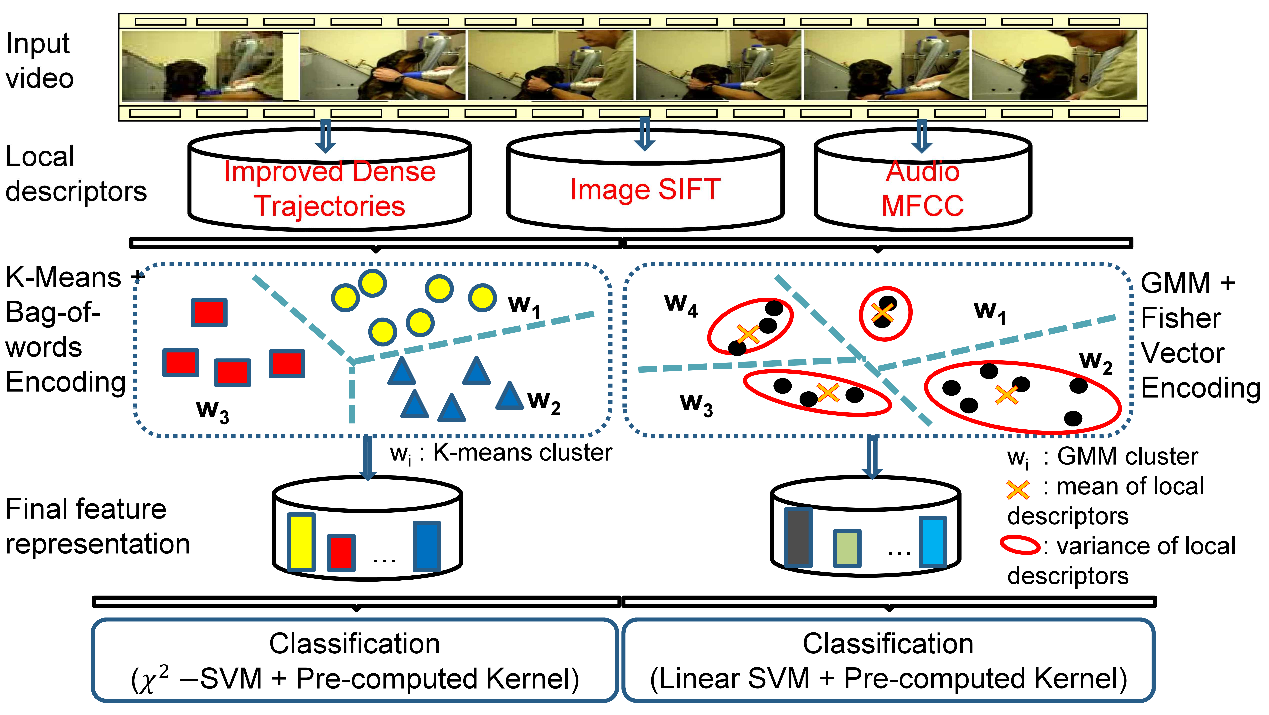
\includegraphics[width=1\textwidth]{framework.pdf}
	\caption{General MED framework}
	\label{med_framework}
\end{figure}

\subsection{Pre-Processing}

The pre-processing component prepares the data for the processing in the other components. First, the video is resized to a width of 320 pixels, and its height is scaled so that the aspect ratio is kept the same. All features are extracted from the resized video. 

To get the image features, keyframes are sampled from the shots at one frames every two seconds. This rate seems to be a good tradeoff between time and accuracy (as suggested in \cite{trecvid10:cuucf}). Blank keyframes, i.e., ones filled with a single color, are removed because they do not contain informative features.

To get the audio features, the audio channel is extracted from the original video and saved as a file in the standard WAV format. The audio features can be extracted from this file.

\subsection{Feature Extraction}

The feature extraction component aims to make a discriminative vector representation for each shot extracted in the pre-processing step. The extraction method depends on what type of feature will be used. To conduct comprehensive evaluations of features for VSD, our framework supports a large variety of features, including global and local visual features. Global features capture the global statistics of each extracted shot. These statistics can be calculated directly from sub regions of a sampled frame and concatenated to form the vector representation for that frame, before being aggregated into the final representation for each shot. It is more complicated to calculate the feature vector representation for local features. The number of local features varies from frame to frame; therefore, it requires a special encoding technique, which will be described in \ref{c2_sec_feature_encoding}.

Besides global and local features, our evaluation framework supports a number of other features. In particular, audio features can be extracted from pre-defined temporal windows. The features of each window provide local audio characteristics at that temporal location. This means audio features can be considered as local. Another kind of feature is a mid-level feature made using concept detectors. We use general concepts taken from off-the-shelf datasets ~\cite{deng2009imagenet}. In addition, our framework supports state-of-the-art deep learning features, which are extracted from a pre-trained model. A description of each feature is presented in Section \ref{c2_sec_med_feature}.

\subsection{Feature encodings}
\label{c2_sec_feature_encoding}

\subsubsection{Bag-of-word model}
As for local features, we use the popular Bag-of-Words (BOW) model to generate a fixed-length representation from local descriptors. This model was initially used to represent text documents \cite{harris1954distributional}, and it was first used to represent images by Csurka et al. \cite{csurka2004visual}. Its extension to motion and audio features is straightforward \cite{sivic2009efficient} and \cite{jiang2010columbia}.

We used the experiment setup described in \cite{jiang2010representations} to make our bag-of-words models. We set the codebook size to 1,000, because in \cite{jiang2010representations}, performance did not significantly improve when the larger codebooks were used, and a smaller codebook can significantly reduce the computational time for feature encoding as well as feature learning. In order to train the codebook, we randomly selected 1 million local descriptors and clustered them using the K-means algorithm. The local descriptors were assigned to each codeword in a soft-weighting manner \cite{jiang2007towards} to improve the discriminative power of the encoded feature.

The main drawback of the bag-of-words model is that it does not incorporate spatial information. The simplest way to overcome this problem is to partition the image into sub-regions and encode local features in each region independently. After that, features from all regions are concatenated into a single feature vector. There are many ways to partition an image into sub-regions. To this end, we follow \cite{jiang2010representations} and \cite{lazebnik2006beyond} and use 2 x 2 and 1 x 3 spatial configurations. We found that these spatial configurations are good trade-offs between performance and computational cost of the high-dimensional feature vector.

\subsubsection{Fisher vector encoding}
The Fisher vector (FV) was first used for image classification in \cite{jaakkola1999exploiting}. It has since been used for action recognition, such as in \cite{sun2013large} and \cite{wang2013action}. Fisher vector encoding can be considered to be an extension of Bag-of-words encoding. Unlike a bag of features, the Fisher vector encodes both first- and second-order statistics between the local descriptors and the codebook. As a result, it is much longer than the BoW feature when using the same codebook. 

\index{fisher vector} \index{bag-of-words} 

Different from bag-of-words encoding, which often uses k-means to train the codebook, the Fisher vector often uses the Gaussian Mixture Model (GMM) to encode the relative position of each local descriptor to each mixture center. The relatively large expressiveness of the Fisher vector means it can achieve comparable performance to that of BoW while using a much smaller codebook \cite{sanchez2013image}, \cite{sun2013large}.

In our experiment, we set the number of Gaussians in the GMM model to K = 256. Then we randomly selected 1,000,000 local descriptors for training the model. As suggested in \cite{perronnin2010improving}, it is better to reduce the local feature dimension by using Principal Component Analysis (PCA). The normalization of the output feature is also very important. Following the recommendation in \cite{perronnin2010improving}, we applied power normalization with $\alpha=0.5$ followed by L2-normalization to the Fisher vector.

\nomenclature[-fv]{FV}{Fisher Vector}
\nomenclature[-pca]{PCA}{Principal Component Analysis}
\nomenclature[-gmm]{GMM}{Gaussian Mixture Model}
\nomenclature[-bow]{BOW}{Bag-of-Words}
\nomenclature[-svm]{SVM}{Support Vector Machines}

\subsection{Learning}

LibSVM \cite{chang2011libsvm} is used for training and testing. For features encoded using the ``bag-of-words'' model, we use the $\chi^2$ kernel to calculate the distance matrix. The optimal (C;g) parameters for learning SVM classifiers are found by conducting a grid search with five-fold cross validation on the original dataset. For features that are encoded with the Fisher vector, we use LibSVM with a linear kernel. In this case, we perform a five-fold cross-validation to obtain the learning parameter C.

\subsection{Fusion Scheme}
Fusing information from different media seems to be a natural way to handle multimedia content. Fusing multi-modal information has been used for multimedia event detection, video search, etc. The different types of multimedia data have their own characteristics, so it is also natural that they would have different fusion strategies. Here, we chose to use late fusion with an average weighting scheme for all features \cite{snoek2005early}.
